\documentclass[a4paper,14pt]{extreport}
\usepackage[left=1.5cm,right=1.5cm,
    top=1.5cm,bottom=2cm,bindingoffset=0cm]{geometry}
\usepackage{scrextend}
\usepackage[T1,T2A]{fontenc}
\usepackage[utf8]{inputenc}
\usepackage[english,russian,ukrainian]{babel}
\usepackage{tabularx}
\usepackage{amssymb}
\usepackage{color}
\usepackage{amsmath}
\usepackage{mathrsfs}
\usepackage{listings}
\usepackage{graphicx}
\graphicspath{ {./images/} }
\usepackage{lipsum}
\usepackage{xcolor}
\usepackage{hyperref}
\usepackage{tcolorbox}
\usepackage{tikz}
\usepackage[framemethod=TikZ]{mdframed}
\usepackage{wrapfig,boxedminipage,lipsum}
\mdfdefinestyle{MyFrame}{%
linecolor=blue,outerlinewidth=2pt,roundcorner=20pt,innertopmargin=\baselineskip,innerbottommargin=\baselineskip,innerrightmargin=20pt,innerleftmargin=20pt,backgroundcolor=gray!50!white}
 \usepackage{csvsimple}
 \usepackage{supertabular}
\usepackage{pdflscape}
\usepackage{fancyvrb}
%\usepackage{comment}
\usepackage{array,tabularx}
\usepackage{colortbl}

\usepackage{varwidth}
\tcbuselibrary{skins}
\usepackage{fancybox}


\usepackage{tikz}
\usepackage[framemethod=TikZ]{mdframed}
\usepackage{xcolor}
\usetikzlibrary{calc}
\makeatletter
\newlength{\mylength}
\xdef\CircleFactor{1.1}
\setlength\mylength{\dimexpr\f@size pt}
\newsavebox{\mybox}
\newcommand*\circled[2][draw=blue]{\savebox\mybox{\vbox{\vphantom{WL1/}#1}}\setlength\mylength{\dimexpr\CircleFactor\dimexpr\ht\mybox+\dp\mybox\relax\relax}\tikzset{mystyle/.style={circle,#1,minimum height={\mylength}}}
\tikz[baseline=(char.base)]
\node[mystyle] (char) {#2};}
\makeatother

\definecolor{ggreen}{rgb}{0.4,1,0}
\definecolor{rred}{rgb}{1,0.1,0.1}
\definecolor{amber}{rgb}{1.0, 0.75, 0.0}
\definecolor{babyblue}{rgb}{0.54, 0.81, 0.94}
\definecolor{amethyst}{rgb}{0.6, 0.4, 0.8}

\usepackage{float}
\usepackage{wrapfig}
\usepackage{framed}
%for nice Code{
\lstdefinestyle{customc}{
  belowcaptionskip=1\baselineskip,
  breaklines=true,
  frame=L,
  xleftmargin=\parindent,
  language=C,
  showstringspaces=false,
  basicstyle=\small\ttfamily,
  keywordstyle=\bfseries\color{green!40!black},
  commentstyle=\itshape\color{purple!40!black},
  identifierstyle=\color{blue},
  stringstyle=\color{orange},
}
\lstset{escapechar=@,style=customc}
%}


\begin{document}
\pagecolor{white}


%----------------------------------------1

\begin{titlepage}
  \begin{center}
    \large
    Національний технічний університет України \\ "Київський політехнічний інститут імені Ігоря Сікорського"


    Факультет Електроніки

    Кафедра мікроелектроніки
    \vfill

    \textsc{ЗВІТ}\\

    {\Large Про виконання курсової роботи \\
      з дисципліни: «Твердотільна електроніка-2»\\[1cm]

        Варіант №50


    }
  \bigskip
\end{center}
\vfill

\newlength{\ML}
\settowidth{\ML}{«\underline{\hspace{0.4cm}}» \underline{\hspace{2cm}}}
\hfill
\begin{minipage}{1\textwidth}
Виконавець:\\
Студент 3-го курсу \hspace{4cm} $\underset{\text{(підпис)}}{\underline{\hspace{0.2\textwidth}}}$  \hspace{1cm}А.\,С.~Мнацаканов\\
\vspace{1cm}

Перевірив: \hspace{6.1cm} $\underset{\text{(підпис)}}{\underline{\hspace{0.2\textwidth}}}$  \hspace{1cm}Л.\,М.~Королевич\\

\end{minipage}

\vfill

\begin{center}
2021
\end{center}
\end{titlepage}

\newpage
\setcounter{page}{2}
\begin{center}
    \textbf{Завдання}
\end{center}
розрахувати порогові напруги транзисторів мікросхеми


\begin{center}
  \textbf{Виконання завдання}
\end{center}

\begin{figure}[h!]
\center{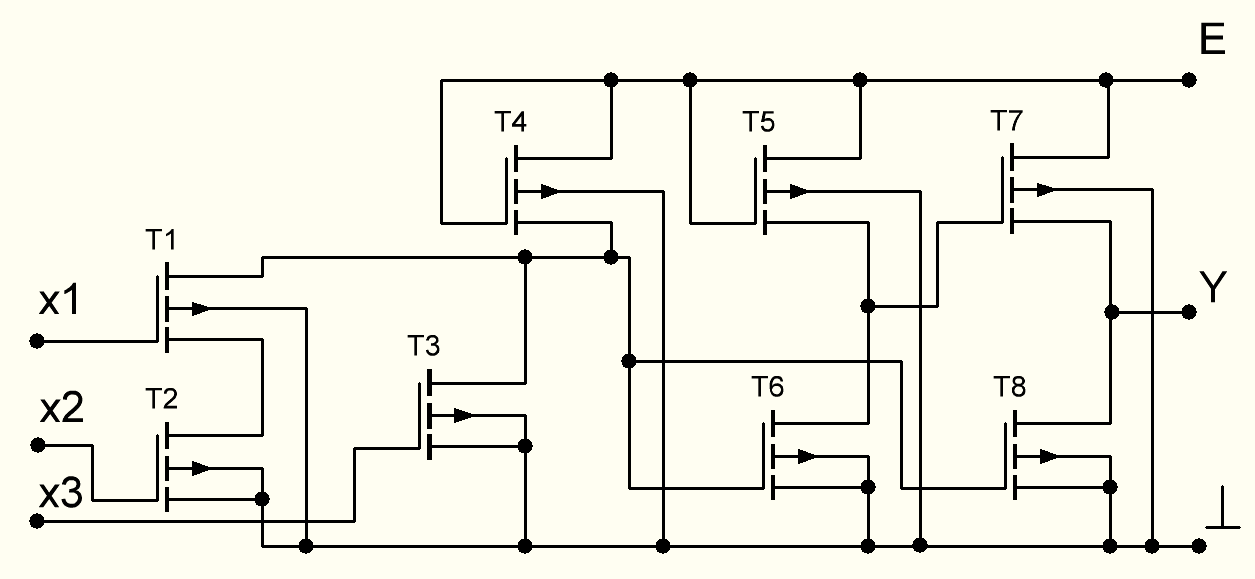
\includegraphics[width=1\linewidth]{1-b.png}}
\caption{Прототип схеми.}
\label{ris1}
\end{figure}

Треба записати формулу для пошуку порогової напруги. За варіантом  у мене КЕФ, тому формула буде наступною:
\begin{equation}
U_{n o p}^{0}=\phi_{M S}-\frac{q \cdot N_{S S}}{C_{o x}}-2 \cdot \phi_{F}-\frac{\sqrt{2 \cdot q \cdot \varepsilon_{0} \cdot \varepsilon_{S} \cdot N_{B}}}{C_{o x}} \cdot \sqrt{\left|2 \cdot \phi_{F}+U_{n}\right|}
\end{equation}

У цій формулі
дано майже все, а точніше: $\quad N_{S S}=7,3 \cdot 10^{11} \text{см}^{-3}$
$\varepsilon_{0}=8,85 \cdot 10^{-14} \Phi / \text{см}$
$q=1,6 \cdot 10^{-19}\text{Кл}$
$k_{B}=1,38 \cdot 10^{-23}$ Дж/К $, T=300 \mathrm{~K}, n_{i}=1,45 \cdot 10^{10} \mathrm{~cm}^{-3}, \varepsilon_{S}=11.8$
Питома ємність шукається як
\begin{equation}
C_{o x}=\varepsilon_{0} \cdot \varepsilon_{o x} / d_{o x}=\frac{8,85 \cdot 10^{-14} \cdot 3,9}{10^{-5}}=3,45 \cdot 10^{-8}\text{ } \frac{\Phi}{\text{см}^{2}}
\end{equation}

Рівень Фермі у об'ємі кремнію:
\begin{equation}
\phi_{F}=\left(\frac{k_{B} \cdot T}{q}\right) \cdot \ln \left(\frac{N_{B}}{n_{i}}\right)
\end{equation}
I невідома сама концентрація $N_{B},$ тому користуємось наступною ф-ю:



\vspace{0.5 cm}
$\sigma=\frac{1}{\rho}=\left.q \cdot n \cdot \mu_{n}\right|_{n=N_{B}} \Rightarrow n=\frac{1}{\rho \cdot q \cdot \mu_{n}}=\frac{1}{5 \cdot 1,6 \cdot 10^{-19} \cdot 1500} \approx 8,3 \cdot 10^{14} \text{ }$ см $^{-3}$
\vspace{0.5 cm}

у формулі бело взято, що $\rho=5$ Ом$\cdot$см$, N_{B}=8,3 \cdot 10^{14}$ \text{ } см$^{-3}$\\

Тобто, рівень Фермі тоді буде:\

$$\phi_{F}=\left(\frac{k_{B} \cdot T}{q}\right) \cdot \ln \left(\frac{N_{B}}{n_{i}}\right)=\frac{1,38 \cdot 10^{-23} \cdot 300}{1,6 \cdot 10^{-19}} \cdot \ln \left(\frac{8,3 \cdot 10^{14}}{1,45 \cdot 10^{10}}\right)=0,283\text{ } B$$\\
За допомогою таблички з методички (сторінка $9,$ таблиця 1) визначив різниця робіт виходу металу затвору і напівпровдникової підкладки, що для моєї концентрації цей параметр буде близько $\phi_{M S}=-0,31 \mathrm{~B} \quad$ (якщо $10^{14}=-0,36,$ а $10^{15}=-0,30,$ то $8.3 \cdot 10^{14}$ прибдизно буде $\left.-0,31\right)$
Тепер треба вказати напруги між витоком і підкладкою для
кожного транзистора, маючи за умовою, що $U^{0}=-1,1 \mathrm{~B} {\text {та }} U^{1}=-10 \mathrm{~B}$. 3а умовою у
мене з +, але так як підкладка КЕФ, то беремо з мінусом.
Якщо витік і підкладка виведені на спільний вивід, то напруга дорівнюватиме нулю. Якщо НЕ підключені до спільного виводу, то там буде логічний нуль (-1.1 В). Але, у мене в схемі транзистор Т1 і Т2 послідовно з'єднані, через що напруга буде розбиватися на два транзистора, і тоді на транзисторі Т1 буде половина напруги логічного нуля.
Тобто:\\


$$
\text{Для } \mathrm{T} 2, \mathrm{~T} 3, \mathrm{~T} 6, \mathrm{~T} 8: U_{n}=0 \text{ } B,  U_{nop}=-4,63\text{ } B
$$
$$
\text{Для } \mathrm{T} 4, \mathrm{~T} 5, \mathrm{~T} 7: U_{n}=-1,1 \text{ }B, U_{\text {nop }}=-4,33 \text{ }B \\
$$
$$
\text{Для Т1: } U_{n}=-1,1 / 2=-0,55 \text{ }B, U_{n o p}=-4,62 \text{ }B
$$

Далі порахуємо «ідеальну» порогову напругу:
$$
U_{\text {\text{ідеал} nop }}=\left(U^{1}+U^{0}\right) / 2=(-10-1,1) / 2=-5,55 \mathrm{~B}
$$
Тепер треба проаналізувати, чи можна такі порогові напруги мати, чи їх треба змінювати (в ідеалі, похибка мусить бути в районі менше $10 \%,$ тоді можена спокійно подавати таку напругу).
Шукаємо абсолютні похибки:\\
$U_{n}=0$\\
$\Delta U_{n o p}=-5,55+4,63=-0,92 \mathrm{~B}$\\
$\delta=100 \cdot|0,92 / 4,63|=20 \%$\\
$U_{n}=-1,1$\\
$\Delta U_{n o p}=-5,55+4,33=-1,22 \mathrm{~B}$\\
$\delta=100 \cdot|1,22 / 4,33|=28 \%$\\
$U_{n}=-0,55$ \\
$\Delta U_{n o p}=-5,55+4,62=-0,93 \mathrm{~B}$ \\
$\Delta U_{\text {nop }}=-5,55+4,62=-0,93 \mathrm{~B}$\\
$\delta=100 \cdot|0,93 / 4,62| \approx 20 \%$\\


Підлеговування треба, тому шукаємо дозу легування за ф-ю $D=\Delta U_{n o p} \cdot C_{o x}$\\
$U_{n}=0$\\
$D=0,92 \cdot 3,45 \cdot 10^{-8} \approx 0,03 \text{ } \text{мкКл} / \text{см}^{2}$\\
$U_{n}=-1,1$\\
$D=1,22 \cdot 3,45 \cdot 10^{-8} \approx 0,04 \text{ } \text{мкКл}  / \text{см}^{2}$\\
$U_{n}=-0,55$\\
$D=0,93 \cdot 3,45 \cdot 10^{-8} \approx 0,03 \text{ } \text{мкКл} / \text{см}^{2}$\\

Ну і далі підлеговуємо. Для цього додаємо до обрахованої порогової доданок:\\
$U_{n}=0$\\
$U_{\text {nop }}^{\prime}=U_{\text {nop }}+\frac{D}{C_{o x}}=-4,63-\frac{0,03}{3,45 \cdot 10^{-8}}=-5,5 \mathrm{~B}$\\
$U_{n}=-1,1$\\
$U_{\text {nop }}^{\prime}=U_{\text {nop }}+\frac{D}{C_{o x}}=-4,33-\frac{0,04}{3,45 \cdot 10^{-8}}=-5,49 \mathrm{~B}$\\
$U_{n}=-0,55$\\
$U_{\text {nop }}^{\prime}=U_{\text {nop }}+\frac{D}{C_{o x}}=-4,62-\frac{0,03}{3,45 \cdot 10^{-8}}=-5,49 \mathrm{~B}$\\

Тут треба ще раз порахувати похибки, побачити, що все входить у межі 10\%. А далі треба сказати, що для того аби зекономити на процесі виготовлення, замість того аби робити два підлегування (з 0.03 і 0.04), можемо зробити одне, для чого візьмемо дозу 0.03, і знову порахуємо напруги (якщо похибка буде менше 10\%, то тоді так і залишаємо, якщо більше, то тоді робимо два підлегування).
Перераховувати для всього не обов’язково, оскільки для першого і третього я і так брав 0.03, тому перерахуємо тільки для 2.

$U_{n}=-1,1$\\

$U_{\text {nop }}^{\prime}=U_{\text {nop }}+\frac{D}{C_{o x}}=-4,33-\frac{0,03}{3,45 \cdot 10^{-8}}=-5,2 \mathrm{~B}$\\

$\delta=100 \cdot|(-5,55+5,2) /(-5,2)|=6,7 \%$\\

Похибка менше $10 \%$ для всіх трьох напруг, тобто достатньо і одного підлегування, що значно спростить технологію виготовлення.

\begin{center}
  \textbf{Висновок}
\end{center}
Стосовно легування, то доза легування не може бути від’ємною, але знак напруги визначатиметься від того, якою домішкою я буду підлеговувати. Тобто, у мене напруги були менші за «ідеальну» порогову напругу, тобто вони були недостатньо «електронні», якщо так можна сказати. Якби у мене порогова напруга була менша за ту, яка вийшла, тоді я мав би підлеговувати акцепторними домішками (p-тип), а оскільки навпаки, то треба n-тип. Поширеними є фосфор і мишьяк, але я обираю фосфор, оскільки він більш поширений (але, усе залежить від того, хто буде проводити цю операцію).

\begin{table}[h]
\begin{tabular}{|c|c|c|}
\hline
№ Транзистора &$ U_{nop}$, \text{[B]} 	& D,	\text{мкКл} / \text{см}$^{2}$ \\ \hline
T1            & -4,62               	& 0,03	\\ \hline
T2            & -4,68               	& 0,03	\\ \hline
T3            & -4,68               	& 0,03	\\ \hline
T4            & -4,33               	& 0,03	\\ \hline
T5            & -4,33               	& 0,03	\\ \hline
T6            & -4,68               	& 0,03	\\ \hline
T7            & -4,33               	& 0,03	\\ \hline
T8            & -4,68               	& 0,03	\\ \hline
\end{tabular}
\end{table}

\end{document}
